\section{Sequenced semantics in a \\ distributed environment}
\label{sec:consider}

\eat{Sequenced semantics has three properties: snapshot reducibility,
extended snapshot reducibility, and change
preservation~\cite{Dignos2012}.  }

Our goal is to enable querying and analysis of large evolving graphs
with sequenced semantics in a distributed environment.  Many
interesting static graphs are so large that they necessitate a
distributed approach, as evidenced by the plethora of works on
Pregel-like computation and graph partitioning~\cite{McCune2015}.
With the added time dimension, efficient computation over graphs with
sequenced semantics presents three challenges:

\begin{enumerate}
\item How to partition temporal relations optimally.
\item How to support sequenced semantics over a partitioned relation.
\item How to partition a large evolving graph such that both temporal
  and structural locality is balanced.
\end{enumerate}

\begin{figure}
\begin{subfigure}[b]{1.6in}
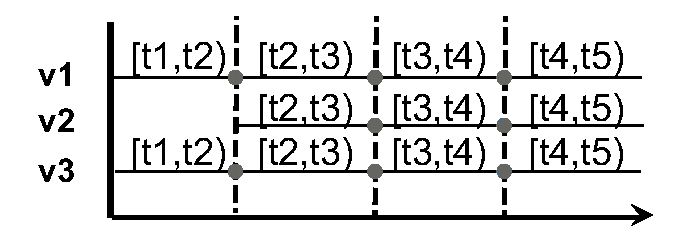
\includegraphics[width=1.6in]{figs/split.pdf}
\caption{with fragments}
\label{fig:split}
\end{subfigure}
\begin{subfigure}[b]{1.6in}
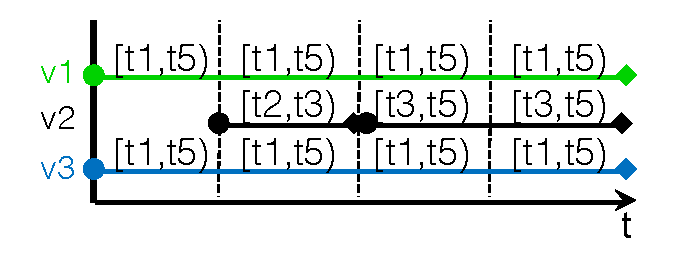
\includegraphics[width=1.6in]{figs/split2.pdf}
\caption{with full timestamps}
\label{fig:split2}
\end{subfigure}
\caption{Relation V from Figure~\ref{fig:coalesced} split in 4 partitions.}
%\vspace{-0.5cm}
\end{figure}

{\bf Temporal partitioning.}  Tuples in a temporal relation can be
divided among the available partitions using time locality.  Following
convention, we refer to the operator that can produce such
partitioning as a {\em splitter}.  The splitter places each tuple into
one or more partitions based on its timestamp.  The goal of the
splitter is to form partitions that are balanced, i.e., have
approximately the same number of items, and require limited
communication between the partitions.  In temporal algebra with point
semantics all queries can be carried out independently at each time
partition, which means that the cross-partition communication is not
necessary.  Recall that snapshot reducibility requires a temporal
operator to produce the same result as if it were evaluated over each
snapshot.  Validity period of a tuple that spans more than one
temporal partition is split, and the tuple is replicated across
partitions.  This increases the overall size of the relation, but all
operations can now be carried out within each partition.  See
Figure~\ref{fig:split} for a simple example of the $V$ relation being
split into four temporal partitions.  Clearly we can carry out a
subgraph operator with predicate \insql{name='Alice'} at each
partition individually.

Temporal partitioning is also appropriate for binary operators as long
as the two input relations are partitioned together, i.e., have the
same splitters.  \eat{Because each entity (vertex or edge) evolves at
  a different rate, the boundaries of partitions will require
  splitting of some of the tuples such that they reside in more than
  one partition.}The question of optimal splitting has been addressed
by Le et al.~\cite{Le2013}, who demonstrated that the relation can be
efficiently split into $k$ buckets in cases of both internal memory
and external memory and guarantee optimality of solution\eat{in $O(N
  log N)$ time in internal memory and in $O(SORT(N)$ I/Os in external
  memory}.  An open question is what to do when a binary operator is
applied to two relations that are already partitioned independently --
it may be more efficient to repartition one of them using the
splitters of the other, or apply the operator over existing partitions
and accept the cost of cross-partition communication.

\eat{As long as the full timestamp is
preserved in each fragment after the split, both the snapshot
reducibility and extended snapshot reducibility properties are
observed using the approach in~\cite{Dignos2012}.}  

{\bf Sequenced semantics over partitioned data.}  Snapshot
reducibility can be guaranteed in the distributed setting, as shown
above.  Extended snapshot reducibility and change preservation require
additional work.  Refer back to Figure~\ref{fig:split} and assume time
granularity of years.  If we perform a subgraph operation with a
temporal predicate such as \insql{p > 2 years} over the split, then we
will get no matches.  However, the original relation contains two
matches -- only Bob with \insql{vid=2} does not meet the predicate.
To assure sequenced semantics over a split relation, we need the full
timestamp of each tuple.  We modify the splitter described above as
follows: during partitioning tuples are placed into their partitions
with their original timestamps.  Incidentally, this is what Le at
al. describe in their work on optimal splitters~\cite{Le2013}.
Provided the full timestamps are preserved during partitioning, the
normalize and align operators from~\cite{Dignos2012} can be carried
out at each partition independently and still produce correct results.
Figure~\ref{fig:split2} shows relation $V$ split in the same four
partitions with this approach.

{\bf Partitioning of graphs.}  Large evolving graphs present
additional challenges compared to static graphs and temporal relations
alone.  Each graph snapshot may be too large to fit into a single
partition.  This necessitates partitioning graphs by both time and
structure.  Miao et al.~\cite{Miao2015} have demonstrated that
different locality, structural or temporal, is more appropriate for
different graph queries.  However, the results do not directly
translate into the distributed environment because of the parallelism
gains.  For instance, they showed that spatial locality provides
better performance than temporal locality in global-point queries,
i.e., queries that compute something over a snapshot for a particular
time point.  In a distributed setting where the communication costs
generally dominate the overall performance, partitioning by time alone
will guarantee that a snapshot is distributed among the lowest number
of partitions.  

Global range queries such as change in graph centrality over time, on
the other hand, are computed over multiple snapshots and their
performance depends on the method of computation.  We can utilize
temporal locality and compute each snapshot independently.  Assuming
that each partition fits one or more snapshots, the maximum number of
snapshots across all partitions will determine the overall
performance.  With structural locality we can distribute edges across
the partitions using any of the already proposed partitioning
approaches such as range- and hash-based~\cite{Seo2013} or the
EdgePartition2D (E2D).  In E2D, a sparse edge adjacency matrix is
partitioned in two dimensions, guaranteeing a $2 \sqrt{n}$ bound on
vertex replication, where $n$ is the number of partitions. E2D has
been shown to provide good performance for Pregel-style
analytics~\cite{DBLP:conf/osdi/GonzalezXDCFS14}.  To minimize
communication with this partition approach caused by the time
dimension, we can use a batching method, effectively computing the
query over all snapshots simultaneously.  

Since the topology of the graph changes over time, the structural
partitioning with the batching method is effective only when the graph
topology changes very little~\cite{MoffittTempWeb16}.  In our
preliminary work we have found that a hybrid approach provides the
best performance even with sub-optimal temporal partitioning.  In the
hybrid approach, graphs are distributed first temporally and then the
batching method is used within each partition.  Alternatively, if the
graphs are too large to fit into a single partition, the partitions
are divided into $k$ buckets where $k$ is a divisor of the total
number of partitions.  Then E2D strategy is used to partition all the
edges within the bucket among the partitions of that bucket.  We are
currently investigating methods for selecting the spatio-temporal
partitioning strategy that provides the best overall performance.
